\documentclass[11pt,a4paper]{article}
\usepackage[T1]{fontenc}\usepackage[utf8]{inputenc}
\usepackage{lmodern,amsmath,amssymb,amsthm,mathtools,booktabs,longtable,array,microtype}
\usepackage[margin=25mm]{geometry}
\setlength{\emergencystretch}{2em}
\usepackage{tikz}\usetikzlibrary{calc}
\usepackage[colorlinks=true,linkcolor=blue,citecolor=blue,urlcolor=blue]{hyperref}
\hypersetup{pdftitle={A deterministic spectral-gap certificate for the spin-2 AKLT model on the kagome lattice},pdfauthor={Anonymous},pdfsubject={Evidence Press v0.3.1 research candidate}}
\newtheorem{theorem}{Theorem}[section]
\newtheorem{lemma}[theorem]{Lemma}\newtheorem{proposition}[theorem]{Proposition}
\newtheorem{corollary}[theorem]{Corollary}
\theoremstyle{remark}\newtheorem{remark}[theorem]{Remark}
\newcommand{\gap}{\operatorname{gap}}\newcommand{\ran}{\operatorname{ran}}
\newcommand{\spec}{\operatorname{spec}}\newcommand{\tr}{\operatorname{tr}}
\newcommand{\rank}{\operatorname{rank}}\newcommand{\id}{\mathbb I}
\newcommand{\Hb}{\widetilde H}\newcommand{\Dstar}{\Delta_*}
\title{A deterministic spectral-gap certificate for the\ spin-2 AKLT model on the kagome lattice}
\author{Anonymous}
\date{Evidence Press research candidate, v0.3.1\\30 September 2026\\\small\url{https://doi.org/10.5281/zenodo.23070704}}
\begin{document}\maketitle
\begin{abstract}
We give a deterministic computer-assisted proof of a uniform spectral gap for the undecorated spin-2 Affleck--Kennedy--Lieb--Tasaki Hamiltonian on kagome tori. With each edge term normalized as the total-spin-four orthogonal projector, the lower bound is
\[
\Dstar=\frac{11(2-\sqrt3)(59-3\sqrt{313})}{3360}>0.0051.
\]
The bound holds on every $m\times n$ torus with $m,n\ge3$, and on a specified class of finite open edge patches formed from unions of down-stars. The natural pairwise overlap test fails. We instead use three-block hubs, combine two blocks before comparing them with the third, and exploit independent dihedral symmetries of the private branches. The required inequalities reduce to 15 pair-sector and 35 triple-sector positive-definiteness tests, the largest of order 11,524. Four further tests, of order at most 856, give an explicit lower bound on the weighted nine-site block gap. Exact rational boundary tensors define the operators; a rank-lift inertia argument avoids certified numerical deflation; every entry of a shifted-Cholesky residual is bounded with outward-rounded error estimates. No random-start assumption or numerical eigenvalue estimate enters acceptance. We specify the Schwinger-polynomial normalization and give exact-integer or rational ordering certificates for the five-spin star gap and elementary-triangle bowtie overlap. The square-lattice conclusion remains a restricted minimal-cross obstruction, not a square-lattice gap proof.
\end{abstract}

\section{Result, contribution and status}
For a finite graph of maximum degree four, place the spin-2 irreducible representation $V_2$ at each vertex and let $P_e$ be the orthogonal projection onto total spin four on the endpoints of $e$. Write
\begin{equation}\label{eq:ham}
 H_\Lambda=\sum_{e\in E(\Lambda)}P_e,\qquad
 \gap(H_\Lambda)=\min(\spec H_\Lambda\setminus\{0\}).
\end{equation}
No rescaling of the edge projector is implicit. The AKLT construction supplies the frustration-free ground spaces~\cite{AKLT}. Guo, Pomata and Wei (GPW)~\cite{GPW} proved gaps for several modified or decorated lattices but left the uniformly spin-2 kagome case open. For the natural kagome down-star cover, they obtained an overlap approximately $0.17067852$, just above the pairwise threshold $1/6$. The present argument retains that cover but changes the local sufficient inequality.

\begin{theorem}[deterministic computer-assisted gap]\label{thm:main}
Let $\Lambda_{m,n}$ be the kagome torus of Section~\ref{sec:geometry}, with $m,n\ge3$. Then
\begin{equation}\label{eq:main}
 \gap(H_{\Lambda_{m,n}})\ge\Dstar
 =\frac{11(2-\sqrt3)(59-3\sqrt{313})}{3360}>\frac{51}{10000}.
\end{equation}
The same bound holds for every nonempty finite down-star edge-union patch defined in Corollary~\ref{cor:patch}.
\end{theorem}

The finite computational assertions supporting this theorem are explicitly stated in Propositions~\ref{prop:angles} and~\ref{prop:blockangle}. Their checkers reconstruct exact inputs and verify all-entry error bounds; they do not merely reread stored scalar results. This is a computer-assisted proof under the documented integer-arithmetic and IEEE/BLAS arithmetic contract, not a proof-assistant formalization. The new proof pipeline has been internally replayed and tested, but has not received external specialist verification.

\paragraph{Methodological scope.}
Local-to-global counting is Knabe-type methodology~\cite{Knabe}; ground-projector compression follows the AKLT overlap approach~\cite{PW,GPW}; verified shifted-Cholesky arguments are established numerical analysis~\cite{Rump}. The contribution here is their specific combination with two-plus-one gluing, the branch symmetry reduction, rational coordinate construction and an explicit end-to-end kagome certificate. We do not claim invention of those general background methods.

Lemm, Sandvik and Wang~\cite{LSW} combine a weighted finite-size criterion with high-precision DMRG for the spin-$3/2$ hexagonal AKLT model. This is a parallel two-dimensional local-to-global precedent, not the spin-2 kagome statement considered here. Rai et al.~\cite{Rai} optimize positive local decompositions in a hierarchy of spectral-gap certificates, encompassing established finite-size bounds; their presentation and numerical demonstrations concern one-dimensional systems. Our construction is a particular kagome-specific sufficient inequality, not a competing general optimization hierarchy. Its sector-dependent two-plus-one grouping changes the sufficient test: the certified pair bound $7/40>1/6$ still cannot pass the earlier pairwise criterion. No comparative SDP benchmark or optimality of our bound is claimed.

\section{Exact polynomial conventions and ground spaces}\label{sec:polynomial}
Let $|k\rangle=|m=2-k\rangle$, $0\le k\le4$, be orthonormal, and set $c_k=\binom4k$. The physical projector is
\begin{equation}\label{eq:P}
 \langle i,j|P|k,l\rangle=
 \mathbf1_{i+j=k+l}\frac{\sqrt{c_ic_jc_kc_l}}{\binom8{i+j}}.
\end{equation}
Two useful rational bases are
\[
 e_k=\frac{|k\rangle}{\sqrt{c_k}},\quad W_e=\operatorname{diag}(1/c_k),
 \qquad b_k=\sqrt{c_k}|k\rangle,\quad W_b=\operatorname{diag}(c_k).
\]
With output $(k,l)$ and input $(i,j)$, the corresponding projector entries are $c_kc_l/\binom8{i+j}$ in the $e$ basis and $c_ic_j/\binom8{i+j}$ in the $b$ basis, subject to equal sums. These matrices are self-adjoint in their respective metrics, not generally in the Euclidean metric.

The Schwinger-polynomial identification used throughout is
\begin{equation}\label{eq:normal}
 u^{4-k}v^k\longmapsto e_k=\frac{|k\rangle}{\sqrt{\binom4k}}.
\end{equation}
In particular, $(u_xv_y-v_xu_y)u_x^3v_y^3$ maps to $|0,4\rangle-\tfrac14|1,3\rangle$, which is annihilated by $P$. The reciprocal convention printed in v0.2 instead produced $|0,4\rangle-4|1,3\rangle$, with overlap $-15/\sqrt{70}$ with the spin-four, magnetization-zero vector. The supplied exact regression rejects that incorrect map.

For an oriented edge put $\omega_{xy}=u_xv_y-v_xu_y$. Changing edge orientation changes only an overall sign in a ground-space map.
\begin{lemma}[ground-space parametrization]\label{lem:vbs}
Let $F$ be a simple edge set on sites $X$, with $\deg_F(x)\le4$. Put $d_x=4-\deg_F(x)$. In convention~\eqref{eq:normal},
\[
 \ker\sum_{e\in F}P_e=
 \left\{\left(\prod_{e\in F}\omega_e\right)q:
 q\in\bigotimes_{x\in X}\mathrm{Poly}_{d_x}(u_x,v_x)\right\}.
\]
The map is injective, its dimension is $\prod_x(d_x+1)$, and it intertwines $\mathrm{SU}(2)$ with the boundary representation $\bigotimes_x V_{d_x/2}$.
\end{lemma}
\begin{proof}
Multiplication by $\omega_{xy}$ is injective from bidegree $(3,3)$ into bidegree $(4,4)$. Its image is the sum of total spins $0,1,2,3$, hence $\ker P_{xy}$. Distinct edge factors are coprime irreducibles in the polynomial ring. Being divisible by every factor is therefore equivalent to divisibility by their product. The remaining degrees are $d_x$, and injectivity follows because the polynomial ring is an integral domain. Each $\omega_e$ is a spin singlet.
\end{proof}

If $\Psi_F$ is the integer coefficient matrix of this multiplication in monomial bases and $W_X=\bigotimes_x\operatorname{diag}(1/c_k)$, then
\begin{equation}\label{eq:gramproj}
 G_F=\Psi_F(\Psi_F^{\mathsf T}W_X\Psi_F)^{-1}\Psi_F^{\mathsf T}W_X
\end{equation}
is the exact ground projector. Its inverse is well-defined by Lemma~\ref{lem:vbs}. This formula, not an approximate eigenspace, defines every projector used below.

\section{Kagome geometry and the hub criterion}\label{sec:geometry}
Label sites $(A,i,j),(B,i,j),(C,i,j)$, with elementary triangles
\[
 U_{ij}=\{(A,i,j),(B,i,j),(C,i,j)\},\quad
 D_{ij}=\{(B,i,j),(A,i+1,j),(C,i+1,j-1)\}.
\]
Every triangle contributes all three edges. Reduce $i$ modulo $m$ and $j$ modulo $n$ for $\Lambda_{m,n}$. A down-star $B_D$ contains a down triangle and its three adjacent up triangles: nine sites and twelve edges. Its weighted Hamiltonian is
\begin{equation}\label{eq:weighted}
 H_D^w=\sum_{e\subset D}P_e+
 \frac13\sum_{\substack{U\text{ meets }D\\e\subset U}}P_e.
\end{equation}
Let $G_D$ be its ground projector, $\Pi_D=\id-G_D$, and $\gamma_0=\gap(H_D^w)$. The block is fixed, so $\gamma_0>0$ independently of volume. On the torus,
\begin{equation}\label{eq:domination}
 H_\Lambda=\sum_D H_D^w\ge\gamma_0\Hb,
 \qquad\Hb=\sum_D\Pi_D,\qquad\ker H_\Lambda=\ker\Hb.
\end{equation}

Each down-star contains three up triangles. Two distinct down-stars meet precisely when they share an up triangle, and then their intersection is that triangle. Each up triangle belongs to three down-stars. To see the unique-pair property, the up-triangle index offsets of $B_{D_{ij}}$ are $(0,0),(1,0),(1,-1)$; their six nonzero ordered differences are distinct modulo $(m,n)$ for $m,n\ge3$. The three stars around $U_{ij}$ have centers $(i,j),(i-1,j),(i-1,j+1)$. Their 21 sites are distinct: for each sublattice the relevant coordinate spans have length at most two. The single-block edge pattern is unchanged under the reduction. These direct coordinate facts are also checked for all $3\le m,n\le8$; the excluded $2\times2$ geometry fails the same test.

\begin{figure}[ht]\centering
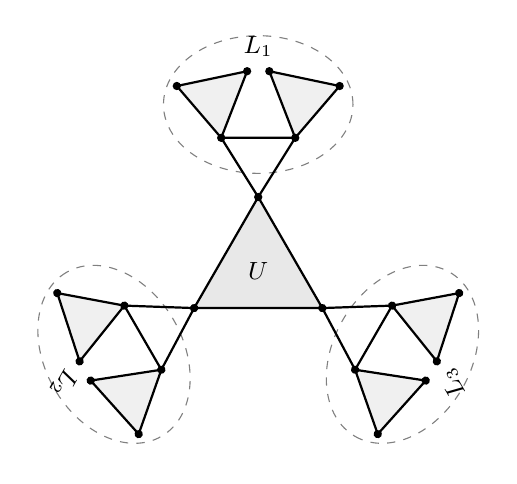
\begin{tikzpicture}[scale=.94,every node/.style={font=\small}]
 \fill[gray!18] (0,1)--({-sqrt(3)/2},-.5)--({sqrt(3)/2},-.5)--cycle;
 \draw[thick] (0,1)--({-sqrt(3)/2},-.5)--({sqrt(3)/2},-.5)--cycle;
 \node at (0,0){$U$};
 \foreach \angle/\r in {0/1,120/2,240/3}{
 \begin{scope}[rotate=\angle]
  \draw[dashed,gray] (0,2.25) ellipse (1.28 and .93);
  \fill[gray!12] (-.5,1.8)--(-1.1,2.5)--(-.15,2.7)--cycle;
  \fill[gray!12] (.5,1.8)--(.15,2.7)--(1.1,2.5)--cycle;
  \draw[thick] (0,1)--(-.5,1.8)--(.5,1.8)--cycle;
  \draw[thick] (-.5,1.8)--(-1.1,2.5)--(-.15,2.7)--cycle;
  \draw[thick] (.5,1.8)--(.15,2.7)--(1.1,2.5)--cycle;
  \foreach \x/\y in {0/1,-.5/1.8,.5/1.8,-1.1/2.5,-.15/2.7,.15/2.7,1.1/2.5}{\fill (\x,\y) circle(1.6pt);}
  \node[rotate=-\angle] at (0,3.03){$L_{\r}$};
 \end{scope}}
\end{tikzpicture}
\caption{The 21-site three-block union, as an abstract local graph. The shared up triangle is $U$; each dashed private region $L_r$ has six sites, two up triangles and the edge joining their connector sites. The nine-site block $B_r=L_r\cup U$ includes the two additional edges from its connector sites to the corresponding vertex of $U$. Each $L_r$ has an independent dihedral symmetry. No edges induced by exterior lattice triangles are added to this union.}\label{fig:hub}
\end{figure}

Set $S_U=\sum_{D:U\subset B_D}\Pi_D$ and $\mu_3=\gap(S_U)$, independent of $U$.
\begin{lemma}[three-block counting]\label{lem:count}
For $m,n\ge3$, $\Hb^2\ge(3\mu_3-2)\Hb$. Thus $\mu_3>2/3$ alone establishes a positive volume-independent gap in~\eqref{eq:ham}.
\end{lemma}
\begin{proof}
Disjoint block projectors commute, so their anticommutators are positive. Each remaining unordered pair belongs to one up-triangle hub. Therefore
\[
 \Hb^2\ge\Hb+\sum_U(S_U^2-S_U)
 \ge\Hb+(\mu_3-1)\sum_US_U=(3\mu_3-2)\Hb.
\]
The last equality uses three hubs per block. Combine with~\eqref{eq:domination} and the common kernel.
\end{proof}

\section{Two-plus-one gluing and spectral localization}\label{sec:gluing}
For orthogonal projections $E,F$, write $E\wedge F$ for their common-range projection and $\vartheta(E,F)=\|EF-E\wedge F\|$. On a nontrivial principal-angle block with cosine $c$, the two positive eigenvalues of $a(\id-E)+(\id-F)$ are
\[
 \frac{a+1\pm\sqrt{(1-a)^2+4ac^2}}2.
\]
The one-dimensional blocks have eigenvalues among $0,a,1,a+1$.
\begin{lemma}[weighted gluing]\label{lem:glue}
Let $G_1,G_2,G_3$ be orthogonal projections, $G_{12}=G_1\wedge G_2$, and $G_{123}=G_1\wedge G_2\wedge G_3$. If
\[
 \vartheta(G_1,G_2)\le\eta<1,\qquad
 \vartheta(G_{12},G_3)\le\theta<1,
\]
then, for $a=1-\eta$,
\begin{equation}\label{eq:glue}
 \gap(3\id-G_1-G_2-G_3)\ge
 g(a,\theta):=\frac{a+1-\sqrt{(1-a)^2+4a\theta^2}}2.
\end{equation}
The same assertion holds separately on invariant sectors, allowing a different choice of the grouped pair on each sector.
\end{lemma}
\begin{proof}
The two-projection decomposition gives $2\id-G_1-G_2\ge a(\id-G_{12})$. Consequently the three-block operator dominates $a(\id-G_{12})+(\id-G_3)$, with the same kernel $\ran G_{123}$. The displayed eigenvalues give~\eqref{eq:glue}; $g(a,\theta)\le a\le1$ also covers the one-dimensional blocks. Orthogonal invariant-sector decompositions preserve operator inequalities and gaps above their respective kernels.
\end{proof}

For the kagome union, $B_r=L_r\cup U$ as in Figure~\ref{fig:hub}. Let $A_X$ denote the projector onto the ground space of the edges internal to $X$. The four regions $L_1,L_2,L_3,U$ are disjoint. Each $A_{L_r}$ commutes with all three $G_i$, satisfies $G_rA_{L_r}=G_r$, and acts disjointly from $G_i$ for $i\ne r$. Also $G_iA_U=G_i$ for all $i$.

\begin{lemma}[localization]\label{lem:local}
If a projection $A$ commutes with $G_1,\ldots,G_p$, and $G_iA=G_i$ for $i$ in a nonempty set $I$, then every eigenvector of $\sum_iG_i$ with eigenvalue $\lambda>p-|I|$ belongs to $\ran A$.
\end{lemma}
\begin{proof}
On $\ker A$, all $G_i$ with $i\in I$ vanish, leaving a sum of at most $p-|I|$ projections.
\end{proof}
Thus every eigenvalue of $S_U$ strictly between zero and one is seen on
\begin{equation}\label{eq:localized}
 \mathcal R=\mathcal V_{L_1}\otimes\mathcal V_{L_2}\otimes\mathcal V_{L_3}\otimes\mathcal V_U,
 \quad \dim\mathcal V_L=3^4\,2^2=324,\quad\dim\mathcal V_U=27.
\end{equation}
The analogous two-block argument captures every nonzero nontrivial pair angle. All these operators commute with $\mathrm{SU}(2)$. The boundary representations have integer total spin, so every multiplet meets total magnetization zero. On $\mathcal R$, that subspace has dimension $106,935,090$.

We do not diagonalize that space. Instead, for pair angles we compress to $\ran G_1$, and for the grouped triple angle to $\ran G_{12}$. Lemma~\ref{lem:vbs} parametrizes these ranges by boundary polynomials. They have ambient coordinate dimensions $81\cdot9\cdot324$ and $81^2\cdot3\cdot324$, respectively, before magnetization and branch symmetry are used. Their common ground spaces are parametrized by $81^2\cdot3$ and $81^3$ boundary coordinates. No induced edge between private regions is imposed merely because it is present in the surrounding lattice.

\section{Dihedral symmetry and exact reduced matrices}\label{sec:reduced}
Number a private branch as triangles $(0,1,2)$ and $(3,4,5)$ joined by edge $(2,5)$. Its residual degrees are $(2,2,1,2,2,1)$. Exchanging sites $0,1$, exchanging $3,4$, and exchanging the two triangles generate $D_8=(S_2\times S_2)\rtimes S_2$. These permutations preserve the exact Gram form. They also intertwine the gluing tensor. On the four external spin-one legs, the corresponding symmetry is the same group.

Let $p$ or $m$ specify the symmetric or antisymmetric part of a pair of spin-one legs; its dimension is six or three. In a private triangle this is tensored with a two-dimensional connector leg, giving dimensions twelve or six. The first sign in $pp,pm,mp,mm$ selects the equal within-triangle parity; the second selects symmetry under exchange of the two triangles. The mixed $pm$ and $mp$ within-triangle parities form two equivalent partners denoted collectively by $x$.
\begin{table}[ht]\centering
\begin{tabular}{lrrr}\toprule
Type $t$ & Private dimension $d_t$ & External dimension $e_t$ & Copies\\\midrule
$pp$ &78&21&1\\$pm$&66&15&1\\$mp$&21&6&1\\$mm$&15&3&1\\$x$&72&18&2\\\bottomrule
\end{tabular}
\caption{Exact branch decomposition. Weighted sums give 324 private and 81 external coordinates. The two $x$ partners are both covered, not discarded.}\label{tab:D8}
\end{table}

For reproducibility, each symmetric/antisymmetric basis consists of columns $e_i\otimes e_j\pm e_j\otimes e_i$ for $i<j$, and $e_i\otimes e_i$ in the symmetric case. No square-root normalization is used. Taking their tensor products and applying the same exchange construction gives Table~\ref{tab:D8}. The checker verifies full rank, exact Gram orthogonality of all six representative/partner spaces, all generating Gram symmetries, and gluing containment, including the second mixed partner. All bases preserve magnetization.

\subsection{Rational frames and contraction formulas}
Expand $\prod_{e\in F}\omega_e$ with integer coefficients. Its Gram matrix has denominator dividing $12^{|X|}$ because $c_k\in\{1,4,6\}$. For the six-site branch, integer accumulation is bounded in absolute value by $12^6 4^7$; the symmetry congruences are bounded by the additional squared column $\ell^1$ norm. The implementation checks that these bounds lie below $2^{62}$ before using signed 64-bit accumulation.

Within each magnetization sector, an exact rational $LDL^{\mathsf T}$ congruence followed by dyadic column scaling makes the private metric diagonal, with entries in $[1,4)$. This is preconditioning by an invertible coordinate change, not an approximation to a square root. The external coordinate frame is similarly rational and magnetization-preserving. The hub Gram matrix $M$ is normalized by a positive rational scalar to have trace 27; that scalar has no effect on its orthogonal projectors.

The two additional singlets joining a private branch to one hub vertex have raw gluing coefficients
\[
 C_{1,1,0}=C_{0,0,2}=1,\qquad
 C_{0,1,1}=C_{1,0,1}=-1,
\]
where the first two indices count down-powers on the connector half-spin legs and the third on the hub spin-one leg; the four external indices are carried unchanged. In a symmetry/frame block, write the resulting exact rational matrices as $C_h\in\mathbb Q^{d_t\times e_t}$, $h=0,1,2$, and the diagonal private metric as $G_L$. Define
\begin{equation}\label{eq:channel}
 D^{(t)}_{a,a',h,h'}=(C_h^{\mathsf T}G_L C_{h'})_{a,a'}.
\end{equation}
For a single block attached at the third hub leg, let $\mathcal C$ embed $e_t\otimes3\otimes3$ into $d_t\otimes3^3$, using $C_h$ on that leg. Put
\begin{equation}\label{eq:localR}
 W=G_L\otimes M,\quad V=W\mathcal C,\quad B_t=\mathcal C^{\mathsf T}V,
 \quad K=VB_t^{-1},\quad R=KV^{\mathsf T}=WG_t.
\end{equation}
The solve $KB_t=V$ is checked exactly. The largest local matrix in this construction is $2106\times2106$, with a 189-column ground map. No floating inverse defines $R$.

For a triple grouping $(t_1,t_2)\mid t_3$, the compressed coordinates are $(a,b,z,c)$: two external indices, one uncontracted hub index, and a private index. Their exact metric and compressed projector form are
\begin{align}
 B_{abzc,a'b'z'c'}&=\delta_{cc'}(G_{L_3})_{cc}
 \sum_{i,i',j,j'}D^{(1)}_{aa'ii'}D^{(2)}_{bb'jj'}M_{ijz,i'j'z'},\label{eq:tripleB}\\
 C_{abzc,a'b'z'c'}&=
 \sum_{i,i',j,j'}D^{(1)}_{aa'ii'}D^{(2)}_{bb'jj'}
 R^{(3)}_{cijz,c'i'j'z'}.\label{eq:tripleC}
\end{align}
Restriction is by the exact condition $m_a+m_b+(1-z)+m_c=0$. The pair formulas omit the second $D$ contraction and leave two hub indices. These formulas are coordinate congruences of a compression of an exact orthogonal projector: $B\succ0$ and $0\preceq C\preceq B$. The eigenvalues of $B^{-1}C$ are the squared principal cosines, including eigenvalue one on the common range.

The common-range count is the number of external tuples with total magnetization zero: $(a,b,y)$ for a pair, with two external indices and one spin-one index, or $(a,b,k)$ for a triple. The external polynomial maps remain injective in every symmetry sector by Lemma~\ref{lem:vbs}. This proves the multiplicity lower bound used in the next section without relying on a numerical rank test.

\subsection{Worked sector: $(mm,mm)\mid mm$}
For this sector, $e_{mm}=3$ and $d_{mm}=15$. The external space is $\bigwedge^2 V_1\cong V_1$; its magnetization character is $\chi_E(t)=t^{-1}+1+t$. The private space is $\bigwedge^2(V_1\otimes V_{1/2})$, with character
\[
 \chi_L(t)=2t^{-2}+3t^{-1}+5+3t+2t^2.
\]
These characters follow directly by adding the weights of distinct pairs in the antisymmetric basis; the rational frames preserve them. Before restricting magnetization, $(a,b,z,c)$ has $3\cdot3\cdot3\cdot15=405$ coordinates. The zero-weight count is
\[
 n=[t^0]\chi_E(t)^3\chi_L(t)
 =3\cdot2+6\cdot3+7\cdot5+6\cdot3+3\cdot2=83.
\]
Here $[t^0]$ denotes the constant coefficient. The common range has
$k=[t^0]\chi_E(t)^3=7$ independent boundary columns, by injectivity of the polynomial map. Thus the checker forms the $83\times83$ pair of exact forms $(B,C)$ in~\eqref{eq:tripleB}--\eqref{eq:tripleC}, chooses an arbitrary dyadic $83\times7$ lift $Y$, and verifies $B/20-C+YY^{\mathsf T}\succ0$. This is the \texttt{(mm,mm)|mm} row of Appendix~\ref{app:sectors}; a separate all-rational small-sector check is described in Section~\ref{sec:certificate}.

The two mixed partners denoted $x$ are exchanged by an exact branch symmetry that intertwines both the Gram form and gluing maps. Applying that symmetry independently on each branch transports the verified inequality to every omitted partner, including products of partners. Hub permutations likewise transport ordered branch placements. They do not force a common grouping across different invariant sectors: each unordered triple receives its recorded grouping, and the resulting operator inequalities combine by orthogonal direct sum.

\subsection{Complete finite verification targets}
The hub has an $S_3$ symmetry permuting its three private branches and hub vertices. Together with Table~\ref{tab:D8}, it leaves 15 unordered pair types and 35 unordered triple types. For each triple type we choose the grouped pair minimizing $e_{t_1}e_{t_2}d_{t_3}$, with a lexicographic tie-break. This is a \emph{sector-dependent} choice. We do not assert a single fixed global grouping has the same bound without checking all its ordered sectors.

\begin{proposition}[validated angle bounds]\label{prop:angles}
The exact pair projectors satisfy $\eta^2<49/1600$. In each triple symmetry sector, the grouping recorded in the certificate table satisfies $\theta^2<1/20$. All 15 pair and 35 triple tests pass the deterministic criterion of Section~\ref{sec:certificate}. The largest pair matrix has order 1894 and the largest triple matrix order 11,524.
\end{proposition}
\begin{proof}[Computer-assisted verification]
Reconstruct the polynomial Grams, rational frames, channels and exact local solves~\eqref{eq:localR}. Assemble~\eqref{eq:tripleB}--\eqref{eq:tripleC}, or their pair versions, with certified error propagation. Apply Lemma~\ref{lem:ranklift} with $q=49/1600$ or $q=1/20$ and the exact common-range count. The program \texttt{run\_validated\_all.py} traverses every unordered type, rejects any failed test, and records all 50 receipts. The exact sector coverage and arithmetic checks are separate from numerical eigenvalue estimates. Appendix~\ref{app:sectors} gives the dimensions and chosen groupings.
\end{proof}
Substitution into Lemma~\ref{lem:glue}, with $a=33/40$, gives
\begin{equation}\label{eq:mu}
 \mu_3\ge\frac{73-\sqrt{313}}{80}>\frac23,
 \qquad 3\mu_3-2\ge\frac{59-3\sqrt{313}}{80}.
\end{equation}
Localization covers the remaining space because its positive spectrum is at least one. This already proves gap existence, without the next section's quantitative block estimate.

\section{A separate small certificate for the nine-site gap}\label{sec:block}
The three up triangles of a down-star are pairwise disjoint. Write $T_0$ for its central down triangle and $G_{T_0}^{\triangle}$ for the triangle ground projector, distinct from the nine-site projector $G_D$ of Section~\ref{sec:geometry}. Let $A=G_{U_1}G_{U_2}G_{U_3}$ and $B=G_{T_0}^{\triangle}$, with identities on omitted sites. Exact rational diagonalization of the three-spin triangle yields
\[
\begin{array}{c|rrrrrrrrr}
\lambda&0&11/14&6/7&69/70&36/35&15/14&10/7&3/2&3\\\hline
\text{multiplicity}&27&18&7&10&5&14&9&22&13.
\end{array}
\]
Hence $\gamma_\triangle=11/14$, and commuting up-triangle projections give
\begin{equation}\label{eq:blockdom}
 H_D^w\ge\frac{11}{14}\left[(\id-B)+\frac13\sum_{j=1}^3(\id-G_{U_j})\right]
 \ge\frac{11}{14}\left[(\id-B)+\frac13(\id-A)\right].
\end{equation}
The last operator and $H_D^w$ have the same kernel.

\begin{proposition}[validated block angle]\label{prop:blockangle}
For these projections, $\vartheta(A,B)^2<2/3$. Consequently
\begin{equation}\label{eq:gamma}
 \gamma_0\ge\frac{11(2-\sqrt3)}{42}>0.07.
\end{equation}
\end{proposition}
\begin{proof}[Computer-assisted verification and deduction]
Compress $B$ to the product of the three up-triangle ground spaces, each parametrized by a 27-column integer polynomial map. Exchanging the two exterior sites of an up triangle splits its boundary space into dimensions 18 and 9. The corresponding common-ground external spaces have dimensions 6 and 3. Permuting the three triangles leaves four unordered parity types. Exact polynomial input, rational frames, the rank-lift lemma and the same all-entry residual validator give the following complete tests.
\begin{center}
\begin{tabular}{lrrr}\toprule
Type&Matrix order&Common dimension&Number of placements\\\midrule
$ppp$&856&38&1\\$ppm$&462&20&3\\$pmm$&252&12&3\\$mmm$&141&7&1\\\bottomrule
\end{tabular}
\end{center}
The weighted dimension sums are 3139 and 141, respectively. All four tests at $q=2/3$ pass. The construction uses $W\Psi(\Psi^{\mathsf T}W\Psi)^{-1}\Psi^{\mathsf T}W$ for the central triangle projector form, and traces the two exterior physical indices of each up-triangle map before contraction. The exact maps are independently checked to lie in every appropriate edge kernel.

The two-projection formula applied to~\eqref{eq:blockdom}, with weights $1$ and $1/3$, gives
\[
 \gamma_0\ge\frac{11}{14}\left(\frac23-\frac1{\sqrt3}\right)
 =\frac{11(2-\sqrt3)}{42}.
\]
\end{proof}
Combining~\eqref{eq:gamma}, \eqref{eq:mu} and Lemma~\ref{lem:count} proves~\eqref{eq:main}. For a rational comparison not relying on displayed decimals, exact squaring gives $\gamma_0>7/100$ and $\mu_3>691/1000$. Thus $\gamma_0(3\mu_3-2)>511/100000>51/10000$.

\section{Deterministic certification and the arithmetic contract}\label{sec:certificate}
\subsection{Rank lift instead of certified deflation}
Numerically subtracting a ground-space projector is unnecessary. The following criterion only needs a proved lower bound on the dimension of the exact common range.
\begin{lemma}[rank-lift inertia certificate]\label{lem:ranklift}
Let $B\succ0$ and $0\preceq C\preceq B$ be real symmetric $n\times n$ matrices. Suppose $B^{-1}C$ has eigenvalue one with multiplicity at least $k$. Let $0<q<1$. If some $n\times k$ matrix $Y$ satisfies
\begin{equation}\label{eq:ranklift}
 qB-C+YY^{\mathsf T}\succ0,
\end{equation}
then eigenvalue one has multiplicity exactly $k$, and every other eigenvalue of $B^{-1}C$ is strictly below $q$.
\end{lemma}
\begin{proof}
The form $qB-C$ has at least $k$ negative eigenvalues, since it is negative on the eigenvalue-one subspace after congruence by $B^{-1/2}$. On $\ker Y^{\mathsf T}$ it is positive by~\eqref{eq:ranklift}. As that kernel has codimension at most $k$, the total dimension of the nonpositive spectral subspace is at most $k$: otherwise it would intersect $\ker Y^{\mathsf T}$ nontrivially. Thus there are exactly $k$ negative eigenvalues and no zero eigenvalues. The asserted generalized eigenvalue ordering follows.
\end{proof}

In the implementation, approximate common vectors $Z$ suggest the lift
\[
 Y\approx\sqrt2\,BZ(Z^{\mathsf T}BZ)^{-1/2}.
\]
The computed $Y$ is simply a finite dyadic matrix with $k$ columns. Its orthogonality, its column span and the accuracy of its construction are \emph{not proof assumptions}. A bad lift can prevent acceptance but cannot invalidate Lemma~\ref{lem:ranklift}. This separates exact geometry from the formerly fragile deflation step.

\subsection{Exact-to-floating representation contract}
All integer polynomial maps, Gram matrices, symmetry maps, rational frames and local inverse factors are constructed exactly. Each conversion to binary64 is checked entry by entry against the original rational number, giving a uniform entry radius. Nonzero rational entries that underflow to zero are rejected. Sparse contraction omits only exact zeros, not entries selected by a tolerance.

The only large operations are sums, products and the candidate Cholesky factorization. The validator assumes conventional binary64 BLAS arithmetic, round to nearest, no overflow, and ordinary dot-product reductions rather than Strassen-like matrix multiplication. Fused multiply-add is admissible. The floating environment and backend identity are recorded. This is an explicit software/hardware trust boundary; it is not removed by the word ``deterministic.''

Put $u=2^{-53}$ and $\widehat\gamma_k=4ku$. For the dimensions here this dominates the conventional relative error bound for a length-$k$ dot product, even if each product and addition is rounded separately. Positive scalar bound operations are rounded outward by \texttt{nextafter}; accumulated positive sums are inflated by $1/(1-\widehat\gamma_k)$. A deliberately oversized absolute allowance $\tau=2^{-900}$ covers underflow in bounded-length operations.

For matrix centers $A_0,B_0$ with uniform entry radii $\epsilon_A,\epsilon_B$, let $r_A\ge\|A_0\|_\infty$, $c_B\ge\|B_0\|_1$, $m_A\ge\max|A_0|$, and $m_B\ge\max|B_0|$. The entry-radius propagation for an inner dimension $k$ is
\begin{align}\label{eq:ballproduct}
 \epsilon_{AB}={}&\widehat\gamma_k\min(r_A m_B,m_A c_B)
 +\epsilon_Ac_B+\epsilon_Br_A+k\epsilon_A\epsilon_B+\tau.
\end{align}
Every right-hand operation is outward bounded. The first term bounds the rounded product of the centers; the remaining terms bound the exact input perturbations. Analogous explicit scalar bounds handle the short channel contractions. Radius row and column sums are retained, so symmetrization gives a spectral-norm radius at most half the sum of their maxima, plus its arithmetic error. The metric product includes the cross term between the private-metric and hub-contraction radii. No sampled residual is substituted for a matrix norm.

\subsection{Every-entry shifted-Cholesky verification}
Let $T=qB-C+YY^{\mathsf T}$ be the exact target, $A_0=A_0^{\mathsf T}$ its computed center, and $e_T\ge\|T-A_0\|_2$. Choose a positive dyadic shift $s$ and compute $S_0=\mathrm{fl}(A_0-s\id)$. Any Cholesky output $L$ is treated as an untrusted candidate factor. The checker computes \emph{every} entry of $S_0-LL^{\mathsf T}$ in row blocks, enclosing all dot-product and subtraction errors. If $e_s$ bounds the diagonal shift error and $r$ bounds the exact residual norm, acceptance requires
\begin{equation}\label{eq:accept}
 s>e_T+e_s+r.
\end{equation}
Indeed $T=LL^{\mathsf T}+s\id+E$ with $\|E\|_2\le e_T+e_s+r<s$, proving positive definiteness. A successful floating Cholesky alone is insufficient. The shifted-residual principle is standard~\cite{Rump}; here its inputs are the exact rational projector forms described above.

For clarity, a bound on the exact maximum squared row norm of $L$ controls every $\sum_j|L_{ij}L_{kj}|$ by Cauchy--Schwarz. Multiplying by $\widehat\gamma_n$ bounds each product residual entry; the checker then bounds a full absolute row sum, not only the largest observed entry. The exact residual is symmetric, so its infinity norm bounds its spectral norm.

For the largest triple test, the recorded dyadic shift is $s=2^{-14}=6.103515625\times10^{-5}$. Its target-construction radius is approximately $4.445\times10^{-7}$ and the total outward error budget is less than $2.976\times10^{-6}$. Thus the certified positive margin exceeds $5.80\times10^{-5}$. These numbers illustrate~\eqref{eq:accept}; the stored JSON contains the full bounds and the replay reconstructs them.

\subsection{Tests, reproducibility and limitations}
The full replay rebuilds the exact tensors, performs all 54 positive-definiteness tests, and reconstructs the exact local results below. It also runs adversarial tests: an indefinite matrix; an insufficient-rank lift; an asymmetric candidate; a deliberately false Cholesky factor; and a too-strong triple bound $\theta^2<3/100$. Each is rejected. A separate 83-dimensional triple calculation is assembled entry by entry over rationals and verified by integer inertia, accepting $1/20$ and rejecting $3/100$. Rational product tests check every entry of their error enclosures, including cancellation and underflow examples. Critical conditions use explicit exceptions, not removable Python assertions; selected checks are replayed with \texttt{python -O}.

The exact local projector factors are rebuilt before use; internal cache files are generated during the run and are not distributed as authoritative proof inputs. The main receipts summarize executions but are not standalone certificates without the code and arithmetic contract. The full replay needs a few gigabytes of memory; the largest validation observed roughly 2.4 GiB resident memory in development. An out-of-memory termination is a failed execution, never an acceptance. The original large numerical filter and its failure-probability estimates are retained privately as historical evidence, not distributed proof inputs. External code review, a second arithmetic implementation, and proof-assistant formalization remain valuable independent assurance steps, not results claimed here.

Publication replay of the unchanged scientific code completed all 20 stages and 54 positive-definiteness tests on macOS ARM64 with NumPy 2.3.5, SciPy 1.17.0, SymPy 1.14.0 and the Accelerate backend in 385.31 seconds. The supplied Linux/OpenBLAS replay is a separate reported record. This is cross-platform implementation replay, not independent reimplementation of the full validator. A supplied separately written small-system checker was also rerun; its exact projector and triangle checks and floating star/bowtie comparisons do not replace full-size validation. These are producer-coordinated checks, not authenticated unaffiliated review.

\section{Finite open edge patches and reusable counting}\label{sec:patch}
\begin{corollary}[uniform gap for down-star edge unions]\label{cor:patch}
Let $\mathcal F$ be any nonempty finite family of down triangles in the infinite kagome lattice. Define the patch sites as $\bigcup_{D\in\mathcal F}B_D$, and its edges as exactly
\[
 E_{\mathcal F}=\bigcup_{D\in\mathcal F}E(B_D).
\]
Then $\gap(\sum_{e\in E_{\mathcal F}}P_e)\ge\Dstar$. The patch need not be connected, and its ground space need not be one-dimensional.
\end{corollary}
\begin{proof}
An up-triangle edge occurs in at most three selected weighted blocks, with weight $1/3$ each; a selected down-triangle edge occurs once with weight one. Hence $H_{\mathcal F}\ge\sum_{D\in\mathcal F}H_D^w\ge\gamma_0\sum_{D\in\mathcal F}\Pi_D$, with the same kernel because exactly the block-union edges are used. Include every up-triangle hub touched by a selected block. Such a hub has one, two or three selected projectors; its gap is at least $1$, $33/40$ or $(73-\sqrt{313})/80$, respectively. All are at least the last value. Each selected block still belongs to exactly three hubs and every intersecting pair to exactly one. The counting proof of Lemma~\ref{lem:count} is unchanged.
\end{proof}
This is an edge-union statement, \emph{not} a claim about arbitrary induced site patches. Adding missing edges changes the kernel and does not justify applying the same gap bound by monotonicity alone. Nor does this paper establish perturbative stability or local topological quantum order. Those stronger properties require further arguments, as illustrated by the hexagonal- and Lieb-lattice results of Jackson, Nachtergaele and Young~\cite{JNY}; their hypotheses and conclusions are not imported here.

More generally, for any family of block projections with $h$ hubs per block, unique-hub intersecting pairs, commuting disjoint blocks, and every active hub sum having gap at least $\mu$, the same expansion gives $\Hb^2\ge[h\mu-(h-1)]\Hb$. The open-patch corollary uses the fact that its truncated hub sums also satisfy the required bound.

\section{Exact small obstructions and spectral ordering}\label{sec:square}
\subsection{Five-spin star}
Let $K=\sum_{j=1}^4P_{0j}$ on a center and four leaves.
\begin{theorem}[exact star gap]\label{thm:star}
\[
 \gap(K)=\alpha=\frac{43-3\sqrt{193}}{28},
\]
the smaller root of $14x^2-43x+2$.
\end{theorem}
\begin{proof}
In magnetization seven, use the seven leaf-orbit sums
\[
(00003),\ (00012),\ (00111),\ (10002),\ (10011),\ (20001),\ (30000)
\]
in the $e$ basis. They have a highest-weight invariant subspace with inclusion, operator and metric
\[
 T=\begin{pmatrix}1/2&3/4&-1/4\\-1/2&-1/4&0\\1&0&0\\0&-3/2&3/4\\0&1&0\\0&0&-3/4\\0&0&1\end{pmatrix},\quad
 A=\begin{pmatrix}5/2&3/2&0\\3/7&13/7&-6/7\\1/7&-3/14&3/14\end{pmatrix},\quad
 B=\begin{pmatrix}7/16&7/16&-1/8\\7/16&17/16&-3/8\\-1/8&-3/8&1/2\end{pmatrix}.
\]
The exact checker verifies $KT=TA$, $BA=A^{\mathsf T}B$, positive leading minors $7/16,35/128,51/512$, and
\[
 \det(x\id-A)=\frac{(2x-3)(14x^2-43x+2)}{28}.
\]
Thus $\alpha\in(0,6/125)$ is an eigenvalue.

For minimality, independently reconstruct the 381-dimensional magnetization-zero physical matrix in the rational $b$ basis. Its positive diagonal metric is $W=\operatorname{diag}(\prod_i c_{k_i})$. The matrix
\[
 7000\,W\left(K-\frac6{125}\id\right)
\]
has integer entries. Exact symmetric fraction-free elimination, checking every division, gives inertia $(336\text{ positive},45\text{ negative},0\text{ zero})$. Lemma~\ref{lem:vbs} gives kernel magnetization-zero dimension 44, the zero-weight multiplicity of four spin-$3/2$ legs. Hence exactly one positive eigenvalue of $K$ lies below $6/125$. It is $\alpha$. Every integer-spin multiplet meets magnetization zero, so this is the global gap. This proof does not depend on supplied characteristic-polynomial factors or floating root ordering.
\end{proof}

\subsection{Minimal square-cross density}
Let $C=\{0,\pm e_1,\pm e_2\}$ in the square lattice and $g_\delta=K^2-\tfrac{1+\delta}{2}K$. On a square torus of side $L$, write $\mathcal T_L(q)=\sum_v\tau_v(q)$.
\begin{lemma}[symmetric density uniqueness]\label{lem:crosskernel}
For one irreducible spin-$s$ representation at each site, a $C$-supported, simultaneously $\mathrm{SU}(2)$- and $D_4$-invariant operator $q$ satisfying $\mathcal T_L(q)=0$ for $L\ge7$ is zero.
\end{lemma}
\begin{proof}
Decompose by exact supports using identity and traceless local operator spaces. Distinct translates of the cross meet in at most two sites, so supports of size at least three cannot cancel. The scalar part vanishes by the trace and each one-site invariant traceless part by Schur's lemma. A two-site invariant operator is a combination of the multiplicity-free pair-spin projectors and is exchange symmetric. Within each translation class of pairs in the cross, placements are related by $D_4$ and have equal coefficients after identification. Their vanishing translation sum forces those coefficients to vanish as well.
\end{proof}
\begin{theorem}[restricted cross obstruction]\label{thm:cross}
For $L\ge7$, a positive semidefinite $C$-supported $q$ with $\mathcal T_L(q)=\mathcal T_L(g_\delta)$ exists if and only if $\delta\le2\alpha-1$. In particular none exists for $\delta\ge0$.
\end{theorem}
\begin{proof}
Average $q$ over $\mathrm{SU}(2)\times D_4$; this preserves positivity, support and the translation-sum constraint. Lemma~\ref{lem:crosskernel} forces the average to equal $g_\delta$. By Theorem~\ref{thm:star}, $g_\delta\succeq0$ exactly when $(1+\delta)/2\le\alpha$. Conversely $q=g_\delta$ then works. For $\delta\ge0$, the fully rational witness $c=(-2,3,5)^{\mathsf T}$ in the displayed star block gives
\[
 c^{\mathsf T}B\left(A^2-\frac{1+\delta}{2}A\right)c
 =-\frac{247}{1568}-\frac{115}{448}\delta<0.
\]
\end{proof}
The relevant identity is
\[
 H^2-\delta H=\sum_v g_\delta^{(v)}+
 \sum_{\{e,f\}:e\cap f=\varnothing}2P_eP_f.
\]
Thus the obstruction concerns the indicated cross density \emph{after disjoint-edge products have been removed}. It does not exclude larger supports, other decompositions or a square-lattice gap.

\subsection{Elementary-triangle bowtie}
Let $E,F$ be ground projections of two triangles sharing one site, embedded in the five-site bowtie.
\begin{proposition}[exact triangle-cover overlap]\label{prop:bowtie}
\[
 \vartheta(E,F)=\frac{47+\sqrt{4417}}{138}.
\]
It exceeds the triangle-cover pairwise threshold $1/3$.
\end{proposition}
\begin{proof}[Exact finite verification]
Construct the triangle polynomial projector~\eqref{eq:gramproj}, embed it on the two triangles, and split the bowtie by its two exterior leaf exchanges and by highest weights. The raising operator in the $e$ basis is $S^+e_k=k e_{k-1}$. Exact nullspaces produce highest-weight blocks of order at most 22. Exact invariance and metric self-adjointness are verified for every block. Their dimensions sum to 381 at magnetization zero and to 3125 after weighting a spin-$J$ block by $2J+1$, so no multiplet is omitted.

Factor each small characteristic polynomial over $\mathbb Q$. Exclude the integer eigenvalues $0,1,2$ algebraically, not by a numerical tolerance. Rational Sturm counts show exactly one distinct noninteger root in $(91/50,2)$; it belongs to $69x^2-185x+108$ and is isolated in $(91/50,183/100)$. Since $0\preceq E+F\preceq2\id$, this is the largest noninteger eigenvalue. It equals $1+\vartheta(E,F)$ by the two-projection decomposition. The magnetization-zero ranks of $E,F$ are 105 each, their common \emph{range} has dimension 19, and their common kernel dimension 190. The full common ground-space dimension is 81.
\end{proof}
A smaller exact witness already gives $\vartheta(E,F)^2\ge55/414>1/9$. The full ordering calculation above establishes the sharper formula while preserving exactness through the final decision.

\section{Positioning, availability and disclosure}
A bounded search on 30 September 2026 checked current web/arXiv discovery and the GPW comparator. It found no competing uniform-gap proof for the same undecorated kagome model. This is not an exhaustive priority review and does not establish worldwide priority. The published GPW figure for the natural kagome cover is Figure 11; numbering differs in the original arXiv version.

The accompanying archive contains the source, replay driver, exact and validated checkers, complete per-sector receipts, logs, reviewer-response table, claim ledger and input provenance. The command \texttt{python code/replay.py} reconstructs the proof calculations. Its \texttt{--quick} mode explicitly does not certify the complete kagome theorem. Requirements and backend details are recorded with the evidence. The manuscript reports neither an external peer-review decision nor an official research-assessment rating.

The investigation and this revision used AI assistance for mathematical derivation, code and drafting. Tests and alternative constructions performed within this workflow are internal checks, not independent external review. No human author is newly named or credited in this candidate. Funding and competing interests: none declared in the supplied materials. Original input archives and their licensing notices are retained privately, with hashes recorded in the public package; original code is supplied under MIT terms and original prose/data under CC0-1.0.

\appendix
\section{Complete sector index}\label{app:sectors}
The following index is generated from the successful full angle replay. For triples, the first two types are the grouped pair and the third is the remaining block. The entry $k$ is the proved common-range count and the number of columns in the dyadic lift. Every pair uses $q=49/1600$ and every triple $q=1/20$. The JSON receipts contain the shift, all outward error bounds, acceptance margin and execution time for each row.
\begin{longtable}{@{}llrrr@{}}
\toprule Mode&Grouping&Order $n$&Common $k$&Error/shift\\\midrule\endfirsthead
\toprule Mode&Grouping&Order $n$&Common $k$&Error/shift\\\midrule\endhead
Pair & \texttt{pp-pp} & 1,894 & 177 & 0.0351 \\
Pair & \texttt{pm-pp} & 1,438 & 137 & 0.0525 \\
Pair & \texttt{pp-mp} & 575 & 58 & 0.0442 \\
Pair & \texttt{mm-pp} & 332 & 33 & 0.0415 \\
Pair & \texttt{x-pp} & 1,770 & 170 & 0.0470 \\
Pair & \texttt{pm-pm} & 1,258 & 105 & 0.0395 \\
Pair & \texttt{pm-mp} & 443 & 46 & 0.0543 \\
Pair & \texttt{mm-pm} & 292 & 25 & 0.0316 \\
Pair & \texttt{pm-x} & 1,438 & 130 & 0.0499 \\
Pair & \texttt{mp-mp} & 194 & 20 & 0.0457 \\
Pair & \texttt{mm-mp} & 109 & 12 & 0.0384 \\
Pair & \texttt{x-mp} & 552 & 58 & 0.0489 \\
Pair & \texttt{mm-mm} & 83 & 7 & 0.0416 \\
Pair & \texttt{mm-x} & 342 & 32 & 0.0394 \\
Pair & \texttt{x-x} & 1,780 & 162 & 0.0350 \\
Triple & \texttt{(pp,pp)|pp} & 11,524 & 1,085 & 0.0487 \\
Triple & \texttt{(pm,pp)|pp} & 8,600 & 803 & 0.0555 \\
Triple & \texttt{(pp,pp)|mp} & 3,389 & 344 & 0.0458 \\
Triple & \texttt{(mm,pp)|pp} & 1,894 & 177 & 0.0361 \\
Triple & \texttt{(pp,x)|pp} & 10,494 & 980 & 0.0484 \\
Triple & \texttt{(pm,pm)|pp} & 6,454 & 607 & 0.0475 \\
Triple & \texttt{(pm,pp)|mp} & 2,547 & 256 & 0.0401 \\
Triple & \texttt{(mm,pm)|pp} & 1,438 & 137 & 0.0421 \\
Triple & \texttt{(pm,x)|pp} & 7,892 & 744 & 0.0359 \\
Triple & \texttt{(mp,pp)|mp} & 1,084 & 112 & 0.0393 \\
Triple & \texttt{(mm,pp)|mp} & 575 & 58 & 0.0446 \\
Triple & \texttt{(pp,x)|mp} & 3,122 & 314 & 0.0592 \\
Triple & \texttt{(mm,mm)|pp} & 332 & 33 & 0.0621 \\
Triple & \texttt{(mm,x)|pp} & 1,770 & 170 & 0.0360 \\
Triple & \texttt{(x,x)|pp} & 9,662 & 914 & 0.0313 \\
Triple & \texttt{(pm,pm)|pm} & 5,616 & 459 & 0.0559 \\
Triple & \texttt{(pm,pm)|mp} & 1,931 & 196 & 0.0463 \\
Triple & \texttt{(mm,pm)|pm} & 1,258 & 105 & 0.0617 \\
Triple & \texttt{(pm,pm)|x} & 6,350 & 564 & 0.0349 \\
Triple & \texttt{(mp,pm)|mp} & 824 & 84 & 0.0455 \\
Triple & \texttt{(mm,pm)|mp} & 443 & 46 & 0.0537 \\
Triple & \texttt{(pm,x)|mp} & 2,374 & 242 & 0.0317 \\
Triple & \texttt{(mm,mm)|pm} & 292 & 25 & 0.0626 \\
Triple & \texttt{(mm,pm)|x} & 1,438 & 130 & 0.0392 \\
Triple & \texttt{(pm,x)|x} & 7,788 & 694 & 0.0610 \\
Triple & \texttt{(mp,mp)|mp} & 358 & 38 & 0.0475 \\
Triple & \texttt{(mm,mp)|mp} & 194 & 20 & 0.0592 \\
Triple & \texttt{(mp,x)|mp} & 1,018 & 104 & 0.0315 \\
Triple & \texttt{(mm,mm)|mp} & 109 & 12 & 0.0443 \\
Triple & \texttt{(mm,x)|mp} & 552 & 58 & 0.0376 \\
Triple & \texttt{(x,x)|mp} & 2,926 & 300 & 0.0559 \\
Triple & \texttt{(mm,mm)|mm} & 83 & 7 & 0.0469 \\
Triple & \texttt{(mm,mm)|x} & 342 & 32 & 0.0591 \\
Triple & \texttt{(mm,x)|x} & 1,780 & 162 & 0.0346 \\
Triple & \texttt{(x,x)|x} & 9,568 & 856 & 0.0418 \\
\bottomrule
\end{longtable}

\section{Verification dependency map}
There are four distinct verification interfaces. \emph{Exact construction} fixes the operators and common-range counts through integer/rational polynomial algebra; correctness of the model-to-code correspondence and the exact-arithmetic libraries is trusted. \emph{Candidate generation} supplies dyadic lift columns and Cholesky factors; their accuracy is not assumed. \emph{Error propagation} encloses all conversions, contractions, symmetrization and residual sums under the stated binary64/BLAS contract. \emph{Final acceptance} checks the strict inequality~\eqref{eq:accept} and complete sector coverage, after which the written gluing and counting argument applies. A fresh execution tests reproducibility of these interfaces, not their independent implementation. The release replay receipt records the backend, source hashes, successful stages and platform; separately reconstructed small systems are corroboration, not a replacement implementation of all 54 tests.
\begin{center}\small
\begin{tabular}{p{.29\textwidth}p{.30\textwidth}p{.32\textwidth}}\toprule
Claim&Analytic dependency&Executable evidence\\\midrule
Exact ground spaces&Polynomial normalization, coprime singlets&\texttt{gram\_exact.py}, \texttt{structural\_checks.py}\\
Reduced projectors&Exact Grams, invertible rational frames&\texttt{rational\_hub.py}\\
Pair and triple angle bounds&Compression, exact common counts, rank-lift lemma&\texttt{certify\_hub.py}, \texttt{run\_validated\_all.py}\\
Positive definiteness&Exact-input error propagation, all-entry residual&\texttt{validated.py}\\
Nine-site block gap&Triangle spectrum, weighted two-projection formula&\texttt{block\_gap.py}, \texttt{exact\_triangle.py}\\
Uniform lattice gap&Hub counting, common kernels&\texttt{structural\_checks.py}, all preceding rows\\
Star minimum&Invariant witness, 44 kernel weights, exact inertia&\texttt{exact\_star.py}, \texttt{star\_inertia.py}, \texttt{inertia.cpp}\\
Bowtie ordering&Complete highest weights, exact factors, Sturm counts&\texttt{bowtie\_certified.py}\\
Adversarial validation&False-input rejection; exact small cross-check&\texttt{validator\_tests.py}\\\bottomrule
\end{tabular}
\end{center}

\section{Version history and ancillary square-threshold correction}
The v0.2 random-start estimates did not bound operator-construction, deflation or rounding errors. Version v0.3 replaced that route by exact inputs and deterministic acceptance. The earlier proposed lower bound $0.0407$ is not established, and the original $106,935,090$-dimensional three-block filter is not a dependency. Version v0.3.1 clarifies sector coverage and verification interfaces, separates triangle and down-star notation, adds methodological comparisons and consolidates this history; it does not change the certified kagome constant.

The GPW weighted-patch threshold is
\[
 t_N(a)=\frac{(N-2)a^2-2(N-2)a+2(N-1)}{2(2N-1)+(N-1)(N-2)a}.
\]
At $a=2,N=34$, $t_{34}(2)/2=33/2246<0.015$. This repairs an earlier threshold comparison, not a patch-gap calculation. No square-lattice patch gap or thermodynamic square-lattice gap follows.

\clearpage
\begin{thebibliography}{9}
\bibitem{AKLT} Affleck, I., Kennedy, T., Lieb, E. H., \& Tasaki, H. (1988). Valence bond ground states in isotropic quantum antiferromagnets. \emph{Communications in Mathematical Physics, 115}, 477--528. \url{https://doi.org/10.1007/BF01218021}
\bibitem{GPW} Guo, W., Pomata, N., \& Wei, T.-C. (2021). Nonzero spectral gap in several uniformly spin-2 and hybrid spin-1 and spin-2 AKLT models. \emph{Physical Review Research, 3}, 013255. \url{https://doi.org/10.1103/PhysRevResearch.3.013255}
\bibitem{Knabe} Knabe, S. (1988). Energy gaps and elementary excitations for certain VBS-quantum antiferromagnets. \emph{Journal of Statistical Physics, 52}, 627--638. \url{https://doi.org/10.1007/BF01019721}
\bibitem{PW} Pomata, N., \& Wei, T.-C. (2020). Demonstrating the Affleck--Kennedy--Lieb--Tasaki spectral gap on 2D degree-3 lattices. \emph{Physical Review Letters, 124}, 177203. \url{https://doi.org/10.1103/PhysRevLett.124.177203}
\bibitem{LSW} Lemm, M., Sandvik, A. W., \& Wang, L. (2020). Existence of a spectral gap in the Affleck--Kennedy--Lieb--Tasaki model on the hexagonal lattice. \emph{Physical Review Letters, 124}, 177204. \url{https://doi.org/10.1103/PhysRevLett.124.177204}
\bibitem{Rai} Rai, K. S., Kull, I., Emonts, P., Tura, J., Schuch, N., \& Baccari, F. (2026). A hierarchy of spectral gap certificates for frustration-free spin systems. \emph{Quantum, 10}, 2065. \url{https://doi.org/10.22331/q-2026-04-13-2065}
\bibitem{JNY} Jackson, T., Nachtergaele, B., \& Young, A. (2026). Local topological quantum order and spectral gap stability for the AKLT models on the hexagonal and Lieb lattices. Preprint, arXiv:2605.12184v3. \url{https://arxiv.org/abs/2605.12184v3}
\bibitem{Rump} Rump, S. M. (2011). Verified bounds for singular values, in particular for the spectral norm of a matrix and its inverse. \emph{BIT Numerical Mathematics, 51}(2), 367--384. Author-hosted full text: \url{https://www.tuhh.de/ti3/paper/rump/Ru10a.pdf}
\end{thebibliography}
\end{document}
